\section{Resultados}

Utilizando el simulador FEM de ADS se obtuvieron los parámetros \textit{S} del filtro analógico utilizando micro strips. El resultado obtenido se muestra en la figura     \ref{fig:resultado_parametros_s}. Se puede observar que el filtro paso-bajo tiene una frecuencia de corte de -3.5 dB a 1.67 GHz.

\begin{figure}[!ht]
    \centering
    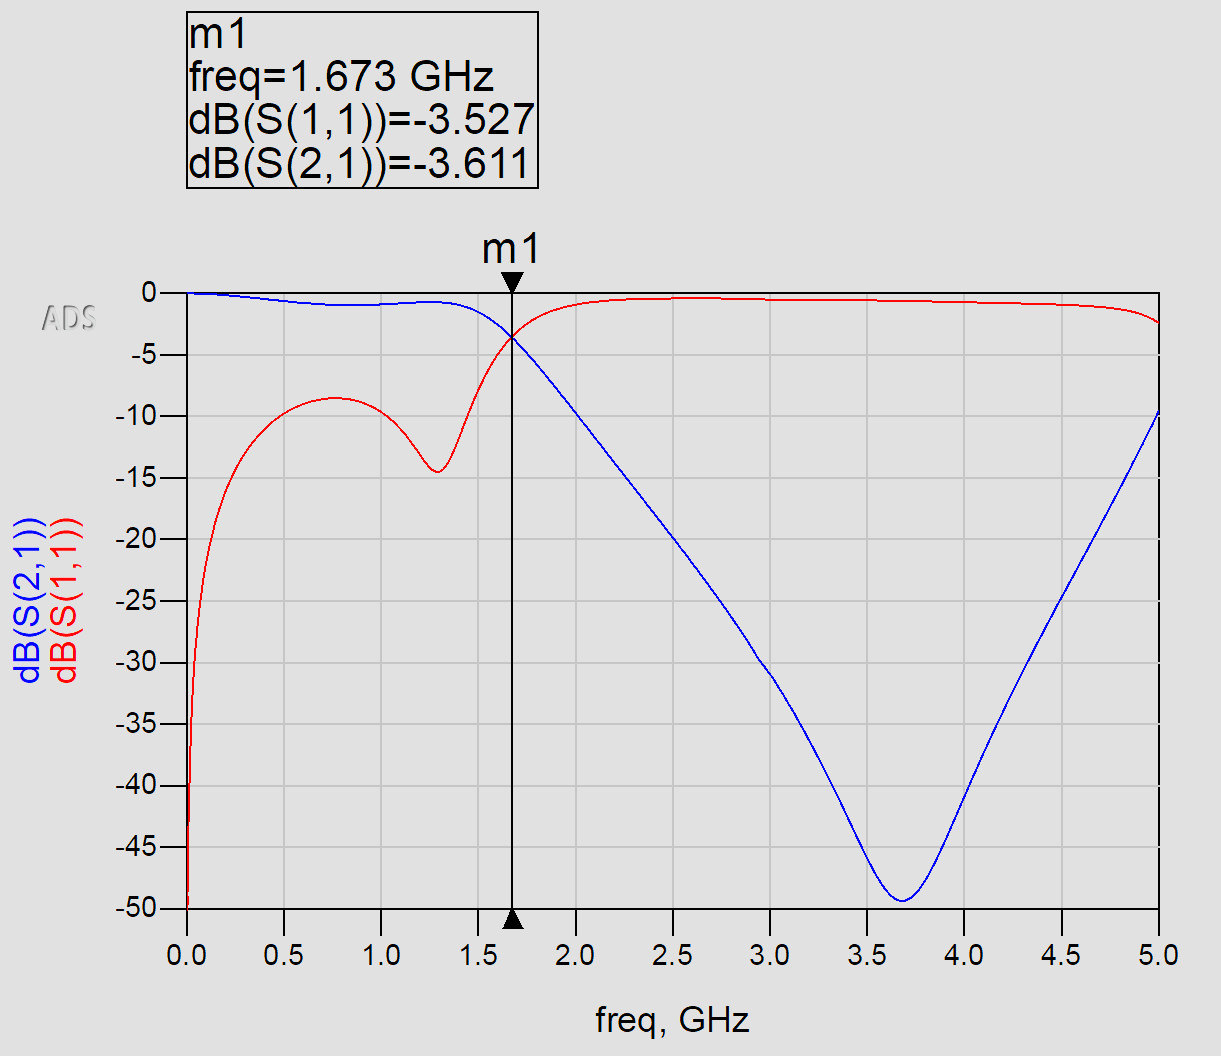
\includegraphics[width=8cm]{figures/resultado.png}
    \caption{Simulación de parámetros S del filtro}
    \label{fig:resultado_parametros_s}
\end{figure}
